\section{Magnetic Fields}

% Magnetic fields

We are interested in modeling the behaviour of the net magnetization,
$\textbf{M}$, of spin packets under the influence of one or more
magnetic fields. This is a function dependent on the time, $t$, and
position, $\textbf{p}$, within the sample. The functions describing
each coordinate component of $\textbf{M}$ are $M_x$, $M_y$ and
$M_z$. Thus our net magnetization is given by

\begin{displaymath}
  \textbf{M}(t, \textbf{p}) = \langle M_x(t, \textbf{p}), M_y(t, \textbf{p}), M_z(t, \textbf{p}) \rangle
\end{displaymath}

As stated previously, when only the static magnetic field
$\mathbf{B}_0 = \langle 0, 0, B_0 \rangle$ is active, $\textbf{M}$
will lie at equilibrium along the z-axis. Thus $\textbf{M} = \langle
0, 0, M_eq \rangle$, where $M_eq$ is the magnitude of $\textbf{M}$.



% Bloch equations
\begin{displaymath}
  \frac{d\mathbf{M}}{dt} = \gamma \mathbf{M} \times \mathbf{B} -
  \frac{\langle M_x, M_y, 0 \rangle}{T_2} - \frac{\langle 0, 0, M_z -
    M_{eq} \rangle}{T_1}
\end{displaymath}

% Magnetic fields

\begin{displaymath}
  \mathbf{B} = \mathbf{B}_0 + \mathbf{B}_1 + \mathbf{B}_G
\end{displaymath}

\begin{displaymath}
  \mathbf{B}_G = \mathbf{B}_{G_s} + \mathbf{B}_{G_\phi} + \mathbf{B}_{G_f}
\end{displaymath}



\subsection{Frequency and phase gradients}

% Constant gradient field along the x axis (read-out direction). The
% strength of the gradient field increases along the x-axis and never
% changes over the course of the signal acquisition.

\begin{displaymath}
  \omega = \gamma (B_0 + x B_{G_f})
\end{displaymath}


% The y-axis is the phase encode direction and is phase encoded with a
% phase gradient.


\begin{figure}
  \centering
  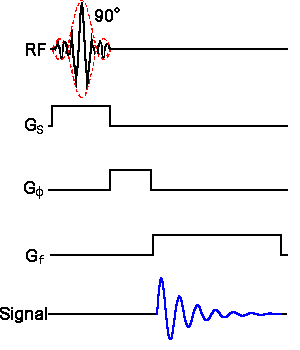
\includegraphics[width=5cm]{gradientSequence}
  \caption{A timing diagram of the application of gradients with
    respect to the RF pulse and signal acquisition.}
  \label{fig:gradientSequence}
\end{figure}


With only the static magnetic field $\mathbf{B}_0 = \langle 0, 0, B_0
\rangle$ and $\mathbf{B}_{G_f} = \langle 0, 0, p_x * B_{G_f} \rangle$
active, the block equations simply to

% Bloch equations with the gradient and B0, which is what we're
% solving

\begin{displaymath}
  \begin{array}{l}
    \frac{dM_x}{dt} = \gamma (B_0 + p_x * B_{G_f}) M_y - \frac{M_x}{T_2} \\
    \frac{dM_y}{dt} = - \gamma (B_0 + p_x * B_{G_f}) M_x - \frac{M_y}{T_2} \\
    \frac{dM_z}{dt} = - \frac{M_z - M_{eq}}{T_1}
  \end{array}
\end{displaymath}



%%% Local Variables:
%%% mode: latex
%%% TeX-master: t
%%% TeX-PDF-mode: t
%%% End:
